\section{RTC - Le réseau téléphonique commuté}

\begin{frame}[fragile]
	\frametitle{Le réseau téléphonique commuté}
\begin{center}
	\Huge{\bf\color{blue}Le réseau téléphonique commuté \\ 
	\LARGE\it PSTN Public Switched telephone Network}
\end{center}
\begin{flushright}
  \item Présentation
  \item La boucle locale
  \item Artères interurbaines (\textit{Backbone})
  \item Les centres de commutations
\end{flushright}
\end{frame}


\begin{frame}[fragile]
  \frametitle{Le réseau téléphonique commuté}
{\large\bf Réseau Téléphonique Commuté (RTC) \\
(\textit{Public Switched Telephone Network (PSTN)}}\\
\textit{«Ce qui coûte le plus cher, c'est de creuser les tranchées»}
\begin{itemize}
	\item Impose de s'appuyer sur RTC
	\item Avec l'arrivée de la fibre, reste encore le problème du «dernier km»
	\item RTC est conçu pour laisser passer la voix ... pas les datas
\end{itemize}
\vspace{1cm}
\textit{Un câble croisé permet le 1Gbit/s, l'ADSL permet 1Mbit/s ... et RTC
(permettait) 56kbit/s}
\end{frame}

\begin{frame}[fragile]
  \frametitle{Le réseau téléphonique commuté}
{\large\bf Structure avec interconnexion totale}
\begin{itemize}
	\item Chaque téléphone est relié à son destinataire.
	\item C'est l'époque de \textit{Graham Bell} (et d'\textit{Elisha Gray}) (1876)
\end{itemize}
\begin{center}
	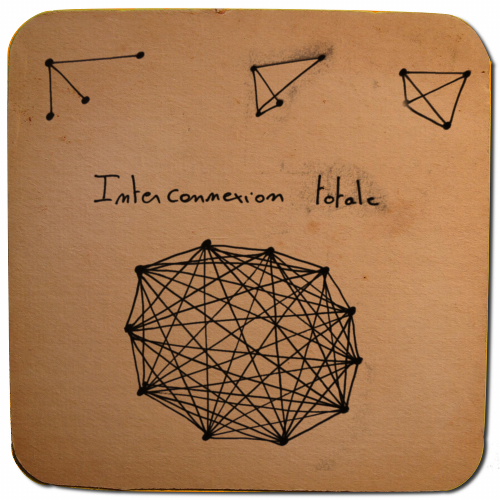
\includegraphics[width=.53\linewidth]{img/sousbock-rtc-interconnexiontotale.png}
	\par{\scriptsize Image de [Tanenbaum]} 
\end{center}
\end{frame}

\begin{frame}[fragile]
  \frametitle{Le réseau téléphonique commuté}
{\large\bf Réseau avec commutateur central}
\begin{itemize}
	\item Chaque téléphone est relié au commutateur central
	\item C'est l'époque de la \textit{Bell Telephone Company} créée par Graham Bell (1878)
\end{itemize}
\begin{center}
	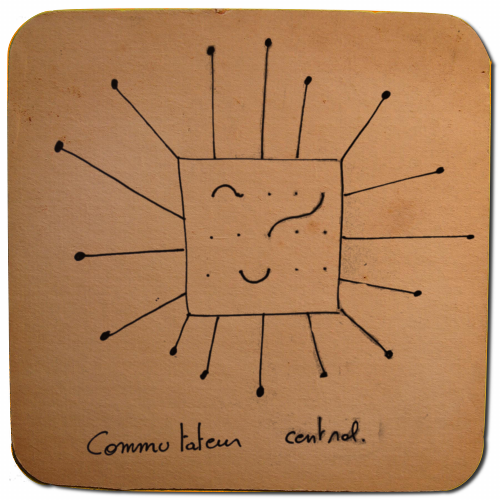
\includegraphics[width=.5\linewidth]{img/sousbock-rtc-commutateurcentral.png}
\end{center}
\end{frame}

\begin{frame}[fragile]
  \frametitle{Le réseau téléphonique commuté}
{\large\bf Réseau hiérarchique à plusieurs niveaux}
\begin{itemize}
	\item Nécessité de connecter plusieurs villes ... apparaissent les centrales
	de second niveau
	\item Système BELL
\end{itemize}
\begin{center}
	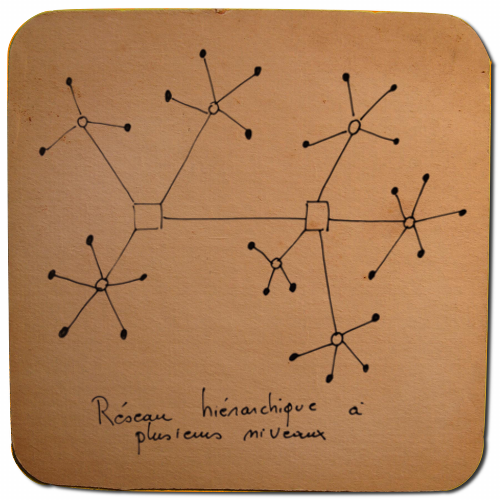
\includegraphics[width=.5\linewidth]{img/sousbock-rtc-hierarchique.png}
\end{center}
\end{frame}

\begin{frame}[fragile]
  \frametitle{Le réseau téléphonique commuté}
{\large\bf Réseau hiérarchique à plusieurs niveaux (avec redondance)}
\begin{itemize}
	\item Permet plusieurs chemins ... \textbf{routage}
\end{itemize}
\begin{center}
	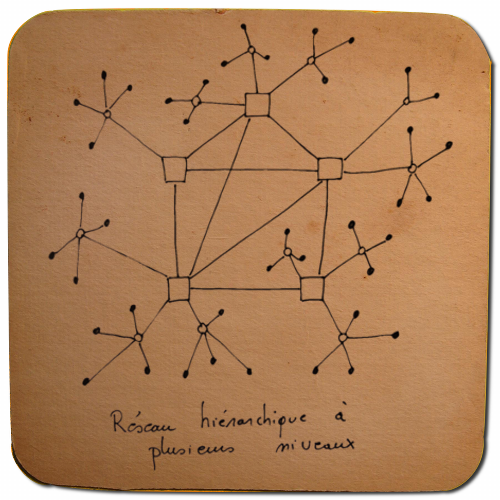
\includegraphics[width=.54\linewidth]{img/sousbock-rtc-hierarchiqueroutage.png}
\end{center}
\end{frame}

\begin{frame}[fragile]
  \frametitle{Le réseau téléphonique commuté}
{\large\bf Les éléments du système téléphonique}
\begin{itemize}
	\item La \textbf{boucle locale (\textit{local loop})}
	\begin{itemize}
		\item longue de 1 à 10km
		\item \textit{relie l'utilisateur au ...}
	\end{itemize}
	\item \textbf{commutateur local (\textit{local central office}) CL}
	\begin{itemize}
		\item paire de fils de cuivre torsadés
		\item si les abonnés sont dans le même central, le CL établit la connexion
		\item \textit{sinon ...}
	\end{itemize}
	\item \textbf{commutateur à autonomie d'acheminement (\textit{Toll office}) CAA}
	\begin{itemize}
		\item deuxième niveau de commutation
		\item forme une ZAA (Zone à autonomie d'acheminement)
		\item reliés aux CL par une \textbf{artère principale (\textit{trunk})}
	\end{itemize}
	\item \textbf{commutateur de transit secondaire (CTS)}
	\begin{itemize}
		\item troisième niveau de commutation
	\end{itemize}
	\item \textbf{commutateur de transit primaire (CTP)}
	\begin{itemize}
		\item quatrième niveau de commutation
	\end{itemize}
\end{itemize}
\end{frame}

\begin{frame}[fragile]
  \frametitle{Le réseau téléphonique commuté}
\begin{center}
	IMG
\end{center}
\end{frame}

\begin{frame}[fragile]
  \frametitle{Le réseau téléphonique commuté}
{\large\bf Évolution historique}
\begin{itemize}
	\item 1984 Fin du monopole de BELL System par le bais du 
	\textit{Modified Final Judgment (\textbf{MFJ})}
	\begin{itemize}
		\item découpage des USA en 164 \textbf{zones d'accès local 
		(LATA \textit{Local Access and Transport Area}}) controlées par un
		opérateur local (\textit{LEC Local Exchange Carrier}
		\item trafic inter-LATA géré par un autre opérateur,
		\textbf{IXC \textit{IntereXchange Carrier}} (AT\&T, Verizon et Sprint)
		\item Pour traiter un appel provenant d'une LATA, un IXC a besoin d'un
		centre de commutation dans la zone appelé \textbf{point de présence (POP
		\textit{Point Of Presence})}
	\end{itemize}
	\item 1996 Fin de la distinction LEC / IXC ... tout le monde peut occuper
	les différents types de marché; câble, téléphonie locale, téléphonie longue
	distance et téléphonie mobile
	\begin{itemize}
	 	\item Corrolaire: portabilité des numéros d'abonné local
	\end{itemize}
	\item 2003 Portabilité des numéros de mobiles
\end{itemize}
\end{frame}

\section{RTC - La boucle locale}

\begin{frame}[fragile]
	\frametitle{La boucle locale}
\begin{center}
	{\Huge\bf\color{blue} La boucle locale}
\end{center}
\end{frame}

\begin{frame}[fragile]
  \frametitle{La boucle locale}
{\large\bf La \textbf{boucle locale} ou \textit{«le dernier kilomètre»}}
\begin{itemize}
	\item Paire de fils de cuivre de l'abonné au \textit{toll office}
	(Commutateur Local ou Commutateur à Autonomie d'Acheminement) 
	\item Nécessite une transformation numérique $\rightarrow$ analogique par le
	biais d'un \textbf{modem}
\end{itemize}
\end{frame}



\section{RTC - Ateliers de recherche 1}

\begin{frame}[fragile]
	\frametitle{RTC - La boucle locale - Ateliers de recherche 1}
{\large\bf Ateliers de recherche 1} 
\begin{itemize}
	\item Sur base des pages 156 à 163 de [Tanenbaum], expliquer, comprendre, … 
	\begin{itemize}
		\item le modem téléphonique
		\item le modem xDSL
		\item la fibre FTTx (\textit{Fibre to the home})
	\end{itemize}
	\item Rédiger un document en groupe pour un des 3 points et le présenter aux autres
	groupes
\end{itemize}
\end{frame}



\section{RTC - Artères interurbaines (backbones)}

\begin{frame}[fragile]
	\frametitle{RTC - Artères interurbaines (backbones)}
\begin{center}
	{\Huge\bf\color{blue} RTC - Artères interurbaines (backbones)}
\end{center}
\end{frame}


\begin{frame}[fragile]
  \frametitle{RTC - Artères interurbaines (\textit{backbones})}
{\large\bf Préalables}
\begin{itemize}
	\item Plusieurs signaux sont \textbf{multiplexés}
	\begin{itemize}
		\item TDM (\textit{time division multiplexing})
		\item FDM (\textit{frequency division multiplexing})
	\end{itemize}
	\item Les boucles locales produisent un signal analogique 
	qui doit être numérisé par un \textbf{codec}
\end{itemize}
\end{frame}

\begin{frame}[fragile]
	\frametitle{RTC - Artères interurbaines (\textit{backbones})}
{\large\bf PCM Pulse Code Modulation} \\
PCM est une technique d'échantillonage
\begin{itemize}
	\item Le codec prélève 8000 échantillons par seconde
	(125 $\mu s$/échantillon)
	\item 8000 échantillons, 2 fois la fréquence de 4000Hz
	\item Chaque échantillon est transformé en nombre de 8 bits
	\item Débit binaire standard 64kbit/s ($2\times4000(Hz)\times8(bits)$)
\end{itemize}
\end{frame}

\begin{frame}[fragile]
	\frametitle{RTC - Artères interurbaines (\textit{backbones})}
{\large\bf Multiplexage temporel}
\begin{itemize}
	\item Envoi de plusieurs signaux en envoyant 1 échantillon de chaque appel toutes les 125$\mu s$
	\item Deux techniques cohabitent
	\begin{itemize}
		\item Technique \textbf{T1}, norme G.733 (États-unis et Japon)
		\item Technique \textbf{E1}, norme G.732 (Europe)
	\end{itemize}
\end{itemize}
\end{frame}

\begin{frame}[fragile]
  \frametitle{RTC - Artères interurbaines (\textit{backbones})}
{\large\bf Multiplexage temporel - Technique T1}
\begin{itemize}
	\item 24 voies téléphoniques multiplexée ensemble
	\item Toutes les 125$\mu s$, une trame est construite en prélevant 8 bits
	sur chaque voie, soit $24\times 8 = 192 bits$ plus 1 bit de contrôle
	\item Une ligne T1 fournit un débit (théorique) de 1,544Mbits/s ($8000\times
	193$) dont 8kbits/s pour la signalisation
	\item Le $193^e$ bit est le \textbf{bit de verrouillage de trame}
\end{itemize}
\end{frame}

\begin{frame}[fragile]
	\frametitle{RTC - Artères interurbaines (\textit{backbones})}
{\large\bf Multiplexage temporel - Technique T1 (suite)}
\begin{center}
	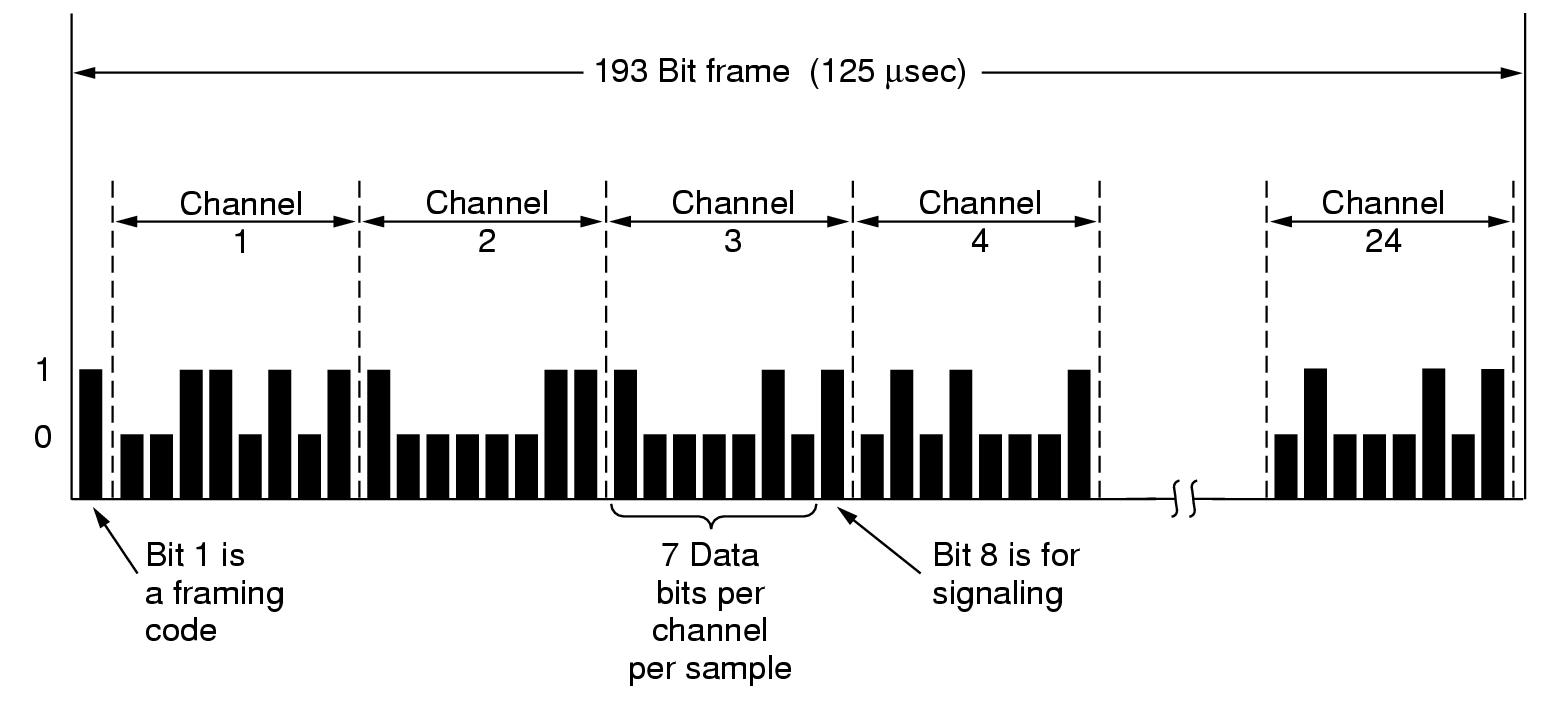
\includegraphics[width=.8\linewidth]{img/2-26-old.jpg}
	\par{\scriptsize Image de [Tanenbaum]} 
\end{center}
\end{frame}

\begin{frame}[fragile]
	\frametitle{RTC - Artères interurbaines (\textit{backbones})}
{\large\bf Multiplexage temporel - Technique E1}
\begin{itemize}
	\item 32 voies téléphoniques multiplexée ensemble
	\item $32\times 8 = 256 bits$
	\item les 8 bits sont utilisés pour les données mais les échantillons 0 et 16 
	sont utilisés pour la signalisation
	\item chaque échantillon est nommé «intervalle de temps» ou \textbf{slot}
	\item une ligne E1 fournit un débit (théorique) de 2,048Mbits/s ($8000\times
	256$) 
\end{itemize}
\end{frame}

\begin{frame}[fragile]
  \frametitle{RTC - Artères interurbaines (\textit{backbones})}
{\large\bf Multiplexage temporel - TDM}
\begin{itemize}
	\item Le multiplexage temporel permet de grouper plusieurs lignes T1 (États-Unis et Japon) 
	ou E1 (Europe)
	\item T1 T2 T3 T4
	\begin{itemize}
		\item T2 = 4 T1 (6.312 Mbits/s)
		\item T3 = 7 T2 (44.736 Mbits/s)
		\item T4 = 6 T3 (274.176Mbits/s)
	\end{itemize}
	\item E1 E2 E3 E4
	\begin{itemize}
		\item E2 = 4 E1 (8.848 Mbits/s)
		\item E3 = 4 E2 (34.304 Mbits/s)
		\item E4 =  4 E3 (139.264 Mbits/s)
	\end{itemize}
\end{itemize}
\end{frame}

\begin{frame}[fragile]
	\frametitle{RTC - Artères interurbaines (\textit{backbones})}
\begin{center}
	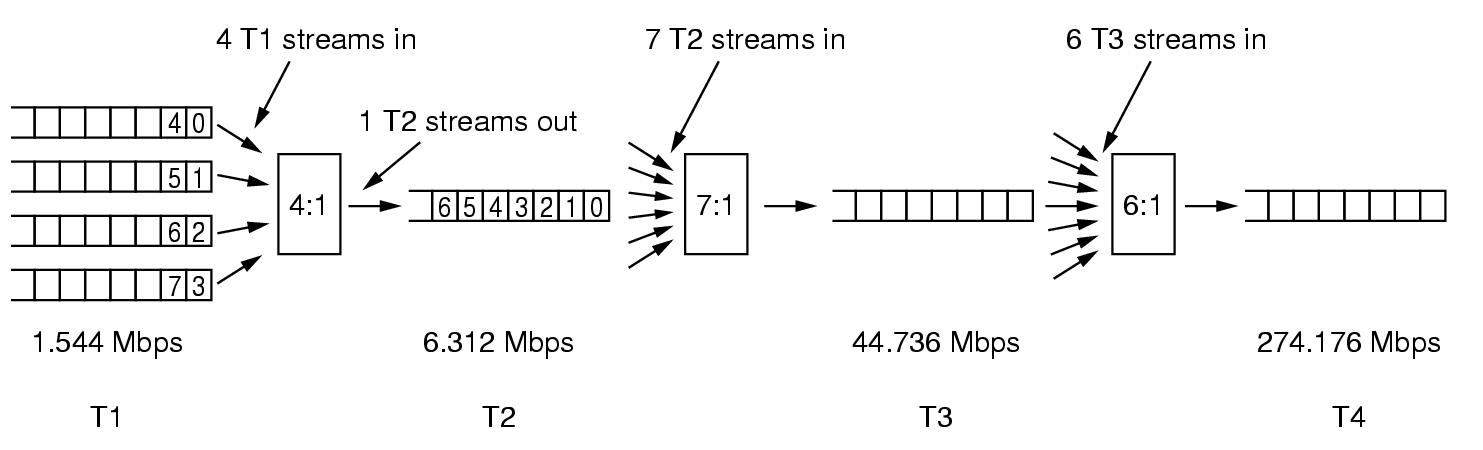
\includegraphics[width=.9\linewidth]{img/2-28-old.jpg}
	\par{\scriptsize Image de [Tanenbaum]} 
\end{center}
\end{frame}



\section{RTC - Ateliers de recherche 2}

\begin{frame}[fragile]
	\frametitle{RTC - Backones - Ateliers de recherche 2}
{\large\bf Ateliers de recherche 2} 
\begin{itemize}
	\item Sur base des pages 167 à 170 de [Tanenbaum], expliquer, comprendre, …
	\textbf{SONET (Synchronous Optical NETwork)}
\end{itemize}
\end{frame}



\section{RTC - Centres de commutation (central office)}

\begin{frame}[fragile]
  \frametitle{RTC - Centres de commutation (central office)}
{\Large\bf RTC - Centres de commutation (central office)}\\
{\large\bf Préalables}
\begin{itemize}
	\item Infrastructure extérieure
	\begin{itemize}
		\item boucle locale (\textit{local loop})
		\item artères principales (\textit{trunk / backbones})
	\end{itemize}
	\item Infrastructure intérieure
	\begin{itemize}
		\item centres de commutation
	\end{itemize}
\end{itemize}
\vspace{.5cm}
Techniques de commutation
\begin{itemize}
	\item commutation de circuits
	\item commutation de paquets
\end{itemize}
\end{frame}

\begin{frame}[fragile]
	  \frametitle{RTC - Centres de commutation (central office)}
{\large\bf Commutation de circuits}
\begin{itemize}
	\item Système téléphonique traditionnel
	\item Principe: recherche d'un chemin de bout en bout avant la transmission des données
	\item Nécessite un délai d'établissement de circuits
	\item Lorsque le chemin est réservé,
	\begin{itemize}
		\item transmission à la vitesse de propagation electromagnétique (5ms/1000km)
		\item pas de congestion
	\end{itemize}
	\item \textbf{Service garanti avec risque de gaspillage de la bande passante}
	\item Facturation à la durée et à la distance
\end{itemize}
\end{frame}

\begin{frame}[fragile]
  \frametitle{RTC - Centres de commutation (central office)}
{\large\bf Commutation de paquets}
\begin{itemize}
	\item Progression grâce à la \textit{voIP}
	\item Les paquets sont envoyés dès qu'ils sont disponibles, ils peuvent
	arriver dans le dérordre
	\item Transmission différée (\textit{store and forward})
	\item Risque de congestion et délai de mise en file
	\item Meilleure tolérance aux pannes (route alternative possible)
	\item \textbf{Service non garanti mais sans gaspillage de bande passante}
	\item Facturation au volume de données
\end{itemize}
\end{frame}

\begin{frame}[fragile]
  \frametitle{RTC - Centres de commutation (central office)}
\begin{center}
	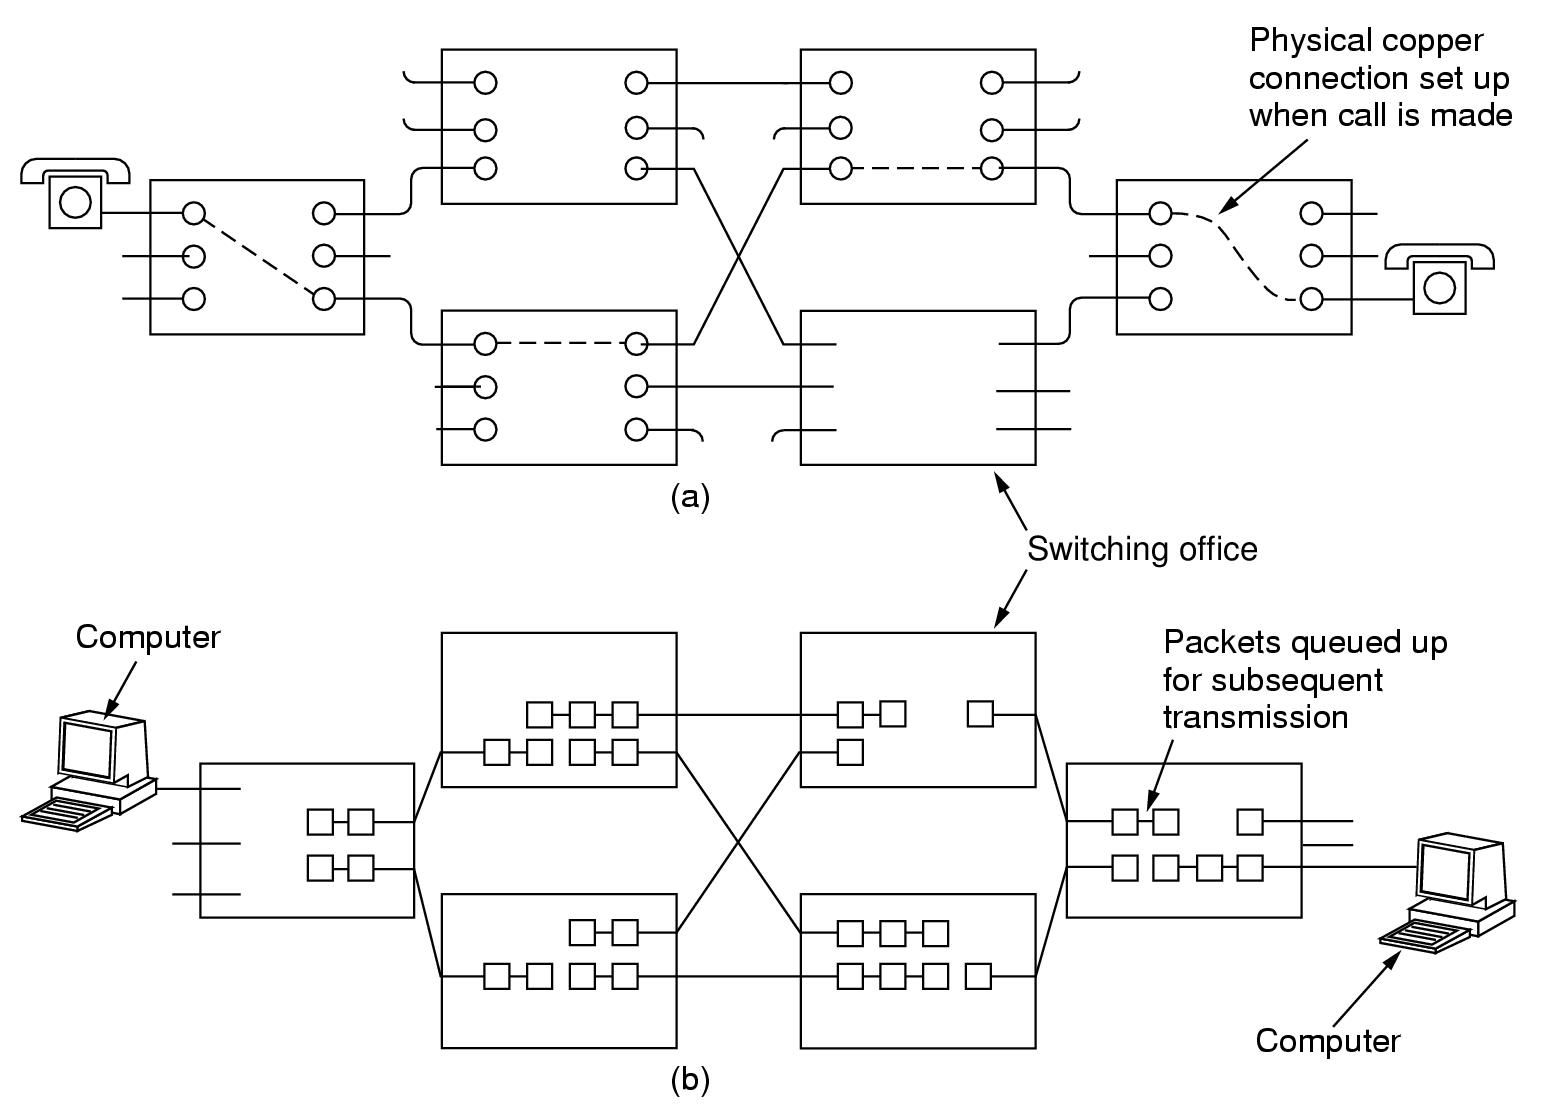
\includegraphics[width=.8\linewidth]{img/2-34-old.jpg}
	\par{\scriptsize (a) Commutation de circuit  (b) Commutation de paquets 
	\\ Image de [Tanenbaum]} 
\end{center}
\end{frame}



\section{RTC - Ateliers de recherche 3}

\begin{frame}[fragile]
	\frametitle{RTC Réseau de télévision câblé - Ateliers de recherche 3}
{\large\bf Ateliers de recherche 3} 
\begin{itemize}
	\item Sur base des pages 192 à 198 de [Tanenbaum], expliquer,
	comprendre,$\cdots$
	\begin{center}
		\textbf{\large le réseau de télévision câblée}
	\end{center}
	\item Rédiger un document commun présentant quelques points de comparaison
	entre \textbf{xDSL} sur le réseau téléphonique commuté et
	l'\textbf{internet par le câble}. 
\end{itemize}
\end{frame}

